\documentclass[11pt]{article}
\usepackage{amsmath}
\usepackage{amssymb}
\usepackage{graphicx}
\usepackage{tabularx}
\usepackage{fancyhdr}
\usepackage{lastpage}

% Page layout
\usepackage[top=1in, bottom=1in, left=1in, right=1in]{geometry}

% Header and footer
\pagestyle{fancy}
\fancyhf{}
\rfoot{Page \thepage}
\renewcommand{\headrulewidth}{0pt}

% Modified Question command with left-aligned number
\newcommand{\questiona}[2]{
    \noindent\textbf{Q#2.} #1 \hfill \textbf{[1 Mark]}
}

\newcommand{\questionb}[2]{
    \noindent\textbf{Q#2.} #1 \hfill \textbf{[2 Marks]}
}

\begin{document}

% Title section with horizontal line
\begin{center}
    \Large\textbf{GATE 2018 - Metallurgical Engineering (MT)} \\
    \large\textbf{General Aptitude and Technical Questions} \\
    \rule{\textwidth}{0.5pt} % Horizontal line below heading
\end{center}

\vspace{0.5cm}


% General Aptitude Section
\section*{General Aptitude}

\questiona{“When she fell down the \_\_\_\_\_, she received many \_\_\_\_\_ but little help.”}{1}
\begin{enumerate}
    \item[(A)] stairs, stares  
    \item[(B)] stairs, stairs  
    \item[(C)] stares, stairs  
    \item[(D)] stares, stares  
\end{enumerate}
\vspace{0.5cm}

\questiona{“In spite of being warned repeatedly, he failed to correct his \_\_\_\_\_ behaviour.”}{2}
\begin{enumerate}
    \item[(A)] rational  
    \item[(B)] reasonable  
    \item[(C)] errant  
    \item[(D)] good  
\end{enumerate}
\vspace{0.5cm}

\questiona{For \(0 \leq x \leq 2\pi\), \(\sin x\) and \(\cos x\) are both decreasing functions in the interval \_\_\_\_\_.}{3}
\begin{enumerate}
    \item[(A)] \( (0, \frac{\pi}{2}) \)  
    \item[(B)] \( (\frac{\pi}{2}, \pi) \)  
    \item[(C)] \( (\pi, \frac{3\pi}{2}) \)  
    \item[(D)] \( (\frac{3\pi}{2}, 2\pi) \)  
\end{enumerate}
\vspace{0.5cm}

\questiona{The area of an equilateral triangle is \(\sqrt{3}\). What is the perimeter of the triangle?}{4}
\begin{enumerate}
    \item[(A)] 2  
    \item[(B)] 4  
    \item[(C)] 6  
    \item[(D)] 8  
\end{enumerate}
\vspace{0.5cm}

\questiona{Arrange the following three-dimensional objects in the descending order of their volumes:

(i) A cuboid with dimensions 10 cm, 8 cm and 6 cm 

(ii) A cube of side 8 cm 

(iii) A cylinder with base radius 7 cm and height 7 cm 

(iv) A sphere of radius 7 cm}{5}
\begin{enumerate}
    \item[(A)] (i), (ii), (iii), (iv)  
    \item[(B)] (ii), (i), (iv), (iii)  
    \item[(C)] (iii), (ii), (i), (iv)  
    \item[(D)] (iv), (iii), (ii), (i)  
\end{enumerate}
\vspace{0.5cm}

\questionb{An automobile travels from city A to city B and returns to city A by the same route. The speed of the vehicle during the onward and return journeys were constant at 60 km/h and 90 km/h, respectively. What is the average speed in km/h for the entire journey?}{6}
\begin{enumerate}
    \item[(A)] 72  
    \item[(B)] 73  
    \item[(C)] 74  
    \item[(D)] 75  
\end{enumerate}
\vspace{0.5cm}

\questionb{A set of 4 parallel lines intersect with another set of 5 parallel lines. How many parallelograms are formed?}{7}
\begin{enumerate}
    \item[(A)] 20  
    \item[(B)] 48  
    \item[(C)] 60  
    \item[(D)] 72  
\end{enumerate}
\vspace{0.5cm}

\questionb{To pass a test, a candidate needs to answer at least 2 out of 3 questions correctly. A total of 6,30,000 candidates appeared for the test. Question A was correctly answered by 3,30,000 candidates. Question B was answered correctly by 2,50,000 candidates. Question C was answered correctly by 2,60,000 candidates. Both questions A and B were answered correctly by 1,00,000 candidates. Both questions B and C were answered correctly by 90,000 candidates. Both questions A and C were answered correctly by 80,000 candidates. If the number of students answering all questions correctly is the same as the number answering none, how many candidates failed to clear the test?}{8}
\begin{enumerate}
    \item[(A)] 30,000  
    \item[(B)] 2,70,000  
    \item[(C)] 3,90,000  
    \item[(D)] 4,20,000  
\end{enumerate}
\vspace{0.5cm}

\questionb{If \(x^2 + x - 1 = 0\), what is the value of \(x^4 + \frac{1}{x^4}\)?}{9}
\begin{enumerate}
    \item[(A)] 1  
    \item[(B)] 5  
    \item[(C)] 7  
    \item[(D)] 9  
\end{enumerate}
\vspace{0.5cm}

\questionb{In a detailed study of annual crow births in India, it was found that there was relatively no growth during the period 2002 to 2004 and a sudden spike from 2004 to 2005. In another unrelated study, it was found that the revenue from cracker sales in India which remained fairly flat from 2002 to 2004, saw a sudden spike in 2005 before declining again in 2006. The solid line in the graph below refers to annual sale of crackers and the dashed line refers to the annual crow births in India. Choose the most appropriate inference from the above data.}{10}

\begin{center}
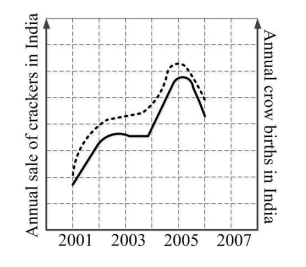
\includegraphics[width=0.5\textwidth]{figures/10.png}
\end{center}

\begin{enumerate}
    \item[(A)] There is a strong correlation between crow birth and cracker sales.  
    \item[(B)] Cracker usage increases crow birth rate.  
    \item[(C)] If cracker sale declines, crow birth will decline.  
    \item[(D)] Increased birth rate of crows will cause an increase in the sale of crackers.  
\end{enumerate}
\vspace{0.5cm}

\section*{Technical Section}

\questiona{For a laminar flow of a liquid metal over a flat plate, the thicknesses of the velocity and thermal boundary layers are \(\delta_v\) and \(\delta_t\) respectively. Kinematic viscosity (viscosity/density) of liquid metal is significantly lower than its thermal diffusivity [thermal conductivity / (density × specific heat)]. Based on this information, pick the correct option. 

(Note: The temperature of the liquid metal is different from that of the plate).}{1}
\begin{enumerate}
    \item[(A)] \(\delta_v < \delta_t\)  
    \item[(B)] \(\delta_v > \delta_t\)  
    \item[(C)] \(\delta_v = \delta_t\)  
    \item[(D)] Information insufficient  
\end{enumerate}
\vspace{0.5cm}

\questiona{What is the most-abundant anion in a \(2CaO \cdot SiO_2\) melt?}{2}
\begin{enumerate}
    \item[(A)] \((SiO_4)^{4-}\)  
    \item[(B)] \((Si_2O_7)^{6-}\)  
    \item[(C)] \((Si_3O_{10})^{8-}\)  
    \item[(D)] \((Si_4O_{14})^{10-}\)  
\end{enumerate}
\vspace{0.5cm}

\questiona{Analysis of a flow phenomenon in a system requires the following variables:  

i. Pressure [M L\(^{-1}\) T\(^{-2}\)]  

ii. Velocity of the fluid [L T\(^{-1}\)]  

iii. Size of the system [L]  

iv. Density of the fluid [M L\(^{-3}\)]  

v. Viscosity of the fluid [M L\(^{-1}\) T\(^{-1}\)]  

According to Buckingham Pi theorem (dimensional analysis), what is the number of independent DIMENSIONLESS variables needed to describe this system?}{3}
\begin{enumerate}
    \item[(A)] 2  
    \item[(B)] 3  
    \item[(C)] 4  
    \item[(D)] 5  
\end{enumerate}
\vspace{0.5cm}

\questiona{In froth flotation, the primary purpose of adding collectors is to:}{4}
\begin{enumerate}
    \item[(A)] make the surface of the mineral hydrophobic.  
    \item[(B)] make the surface of the mineral hydrophilic.  
    \item[(C)] stabilize the froth.  
    \item[(D)] adjust the pH.  
\end{enumerate}
\vspace{0.5cm}

\questiona{Arrange the following in the correct sequence of operations in an integrated steel plant:

i. Basic Oxygen Furnace (BOF)  

ii. Blast Furnace (BF)  

iii. Ruhrstahl Heraeus Degassing Process (RH)  

iv. Ladle Furnace Process (LF)}{5}
\begin{enumerate}
    \item[(A)] BOF \(\rightarrow\) BF \(\rightarrow\) LF \(\rightarrow\) RH  
    \item[(B)] BF \(\rightarrow\) LF \(\rightarrow\) BOF \(\rightarrow\) RH  
    \item[(C)] RH \(\rightarrow\) LF \(\rightarrow\) BF \(\rightarrow\) BOF  
    \item[(D)] BF \(\rightarrow\) BOF \(\rightarrow\) LF \(\rightarrow\) RH  
\end{enumerate}
\vspace{0.5cm}

\questiona{During decarburization in a steel bath at 1550\(^\circ\)C, the compositions of dissolved C (wt.\%C) and dissolved O (wt.\%O) follow the relation:  

\[(\text{wt.\%C})(\text{wt.\%O}) = K\]

When the partial pressure of CO (\(p_{CO}\)) is 1 atm, \(K = 0.002\).  

If \(p_{CO} = 0.1\) atm, what is the value of \(K\), at the same temperature?  

Note: Assume Henry’s law is applicable.}{6}
\begin{enumerate}
    \item[(A)] 0.06  
    \item[(B)] 0.002  
    \item[(C)] 0.02  
    \item[(D)] 0.0002  
\end{enumerate}
\vspace{0.5cm}

\questiona{During upset forging, and considering friction, which of the following profiles represents the axial compressive stress?

Note: In these profiles, the absolute value of the axial compressive stress is plotted on the y-axis.}{7}
\begin{center}
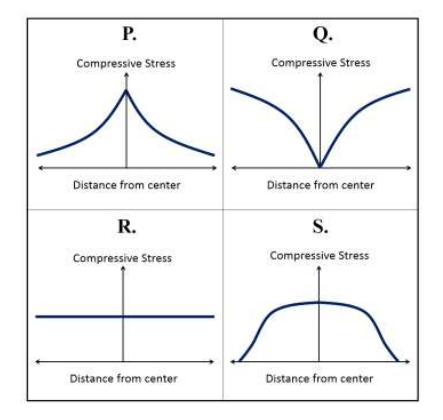
\includegraphics[width=0.5\textwidth]{figures/7.png}
\end{center}
\begin{enumerate}
    \item[(A)] P  
    \item[(B)] Q  
    \item[(C)] R  
    \item[(D)] S  
\end{enumerate}
\vspace{0.5cm}

\questiona{Consider the following engineering components:  

P. Gas turbine blades  

Q. Tungsten-based heavy alloy penetrators  

R. Self-lubricating bearings  

S. Engine block of an automobile  

Which of the following two components are produced by powder metallurgy?}{8}
\begin{enumerate}
    \item[(A)] P \& Q  
    \item[(B)] Q \& R  
    \item[(C)] Q \& S  
    \item[(D)] P \& S  
\end{enumerate}
\vspace{0.5cm}

\questiona{Which of the following materials are protected by passivation (i.e., formation of a thin adherent film on the surface) from corrosion?  

P. Aluminium alloys  

Q. Mild steel  

R. Stainless steel  

S. Silver}{9}
\begin{enumerate}
    \item[(A)] P \& Q  
    \item[(B)] Q \& R  
    \item[(C)] Q \& S  
    \item[(D)] P \& R  
\end{enumerate}
\vspace{0.5cm}

\questiona{The \(c/a\) ratio of Zn (hcp) is 1.856. Slip at room temperature occurs most easily on which of the following slip systems in Zn:  

Note: In hcp metals, the ideal \(c/a\) ratio is 1.633.}{10}
\begin{enumerate}
    \item[(A)] \(\{11\bar{2}0\} \langle 1\bar{1}00 \rangle\)  
    \item[(B)] \(\{11\bar{2}0\} \langle 0002 \rangle\)  
    \item[(C)] \(\{0001\} \langle 11\bar{2}0 \rangle\)  
    \item[(D)] \(\{10\bar{1}1\} \langle 11\bar{2}3 \rangle\)  
\end{enumerate}
\vspace{0.5cm}

\questiona{At equilibrium, the maximum number of phases in a three-component system at CONSTANT PRESSURE is:}{11}
\begin{enumerate}
    \item[(A)] 1  
    \item[(B)] 2  
    \item[(C)] 3  
    \item[(D)] 4  
\end{enumerate}
\vspace{0.5cm}

\questiona{For a single phase system with \(K\) components, the exact differential of Gibbs free energy is given as:  

\[
dG = -S\,dT + V\,dP + \sum_{i=1}^{K} \mu_i\,dn_i
\]

Which one of the following can be derived from the above expression as a Maxwell’s relation?}{12}
\begin{enumerate}
    \item[(A)] \(\left( \frac{\partial S}{\partial P} \right)_{T, n_i} = -\left( \frac{\partial V}{\partial T} \right)_{P, n_i}\)  
    \item[(B)] \(\left( \frac{\partial S}{\partial V} \right)_{T, n_i} = \left( \frac{\partial V}{\partial T} \right)_{P, n_i}\)  
    \item[(C)] \(\left( \frac{\partial S}{\partial T} \right)_{T, n_i} = -\left( \frac{\partial V}{\partial P} \right)_{T, n_i}\)  
    \item[(D)] \(\left( \frac{\partial S}{\partial P} \right)_{T, n_i} = \left( \frac{\partial V}{\partial P} \right)_{T, n_i}\)  
\end{enumerate}
\vspace{0.5cm}

\questiona{For intrinsic Si at room temperature, the electron concentration = the hole concentration = \(1 \times 10^{16} \text{ m}^{-3}\), and the electron and hole mobilities are 0.1 and 0.2 \(\text{m}^2/\text{V}\cdot\text{s}\) respectively. What is the room temperature electrical conductivity?  

The charge of an electron is \(1.6 \times 10^{-19}\,\text{C}\).}{13}
\begin{enumerate}
    \item[(A)] 0 \((\Omega\cdot\text{m})^{-1}\)  
    \item[(B)] \(1.6 \times 10^{-4} (\Omega\cdot\text{m})^{-1}\)  
    \item[(C)] \(3.2 \times 10^{-4} (\Omega\cdot\text{m})^{-1}\)  
    \item[(D)] \(4.8 \times 10^{-4} (\Omega\cdot\text{m})^{-1}\)  
\end{enumerate}
\vspace{0.5cm}

\questiona{To minimize refractory loss during BOF steel-making, slag is supersaturated with which of the following:}{14}
\begin{enumerate}
    \item[(A)] \(Al_2O_3\)  
    \item[(B)] \(Fe_2O_3\)  
    \item[(C)] \(SiO_2\)  
    \item[(D)] \(MgO\)  
\end{enumerate}
\vspace{0.5cm}

\questiona{Which of the following welding processes is NOT suitable for joining thin metal sheets?}{15}
\begin{enumerate}
    \item[(A)] Gas Metal Arc Welding  
    \item[(B)] Electro Slag Welding  
    \item[(C)] Electron Beam Welding  
    \item[(D)] Laser Beam Welding  
\end{enumerate}
\vspace{0.5cm}

\questiona{Which of the following categories of materials is suitable as a filler for brazing of steel sheets?}{16}
\begin{enumerate}
    \item[(A)] Epoxy resins  
    \item[(B)] Near-eutectic alloys  
    \item[(C)] Refractory alloys  
    \item[(D)] Large freezing range alloys  
\end{enumerate}
\vspace{0.5cm}

\questiona{Arrange the following processes in INCREASING magnitude of surface roughness of the casting:  

P. Investment casting  

Q. Permanent mould casting  

R. Pressure die casting  

S. Sand casting}{17}
\begin{enumerate}
    \item[(A)] $R < S < Q < P $ 
    \item[(B)] $P < S < Q < R  $
    \item[(C)] $R < P < Q < S $ 
    \item[(D)]$ Q < P < R < S  $
\end{enumerate}
\vspace{0.5cm}

\questiona{In a Jominy end-quench test of the eutectoid plain-carbon steel, which of the following represents the sequence of microstructures observed from the quenched end of the specimen?}{18}
\begin{enumerate}
    \item[(A)] Fine Pearlite, Coarse Pearlite, Martensite and Pearlite, Martensite  
    \item[(B)] Martensite, Martensite and Pearlite, Fine Pearlite, Coarse Pearlite  
    \item[(C)] Coarse Pearlite, Pearlite and Martensite, Fine Pearlite, Martensite  
    \item[(D)] Martensite, Martensite and Pearlite, Coarse Pearlite, Fine Pearlite  
\end{enumerate}
\vspace{0.5cm}

\questiona{A long oil pipeline made of steel is suspected to have developed a scale on the inner surface due to corrosion. Which of the following non-destructive techniques is the most suitable for detecting and quantifying such a defect?}{19}
\begin{enumerate}
    \item[(A)] Dye penetrant test  
    \item[(B)] Magnetic particle inspection  
    \item[(C)] Ultrasonic inspection  
    \item[(D)] Acoustic emission  
\end{enumerate}
\vspace{0.5cm}

\questiona{A steel is plastically worked in the temperature range below the nose of the TTT curve and above \(M_s\), followed by quenching to produce fine martensite. What is this process called?}{20}
\begin{enumerate}
    \item[(A)] Martempering  
    \item[(B)] Ausforming  
    \item[(C)] Inter-critical forming  
    \item[(D)] Normalizing  
\end{enumerate}
\vspace{0.5cm}

\questiona{What is the requirement for equilibrium at a triple junction as shown in the schematic, with \(\gamma_{12}, \gamma_{23}\) and \(\gamma_{13}\) as grain boundary tensions and \(\theta_1, \theta_2\) and \(\theta_3\) as dihedral angles?}{21}
\begin{center}
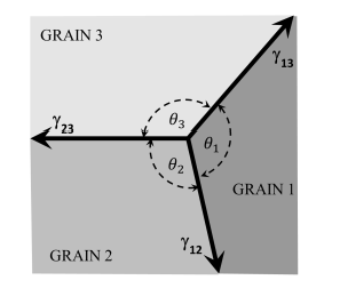
\includegraphics[width=0.5\textwidth]{figures/21.png}
\end{center}
\begin{enumerate}
    \item[(A)] \(\frac{\gamma_{23}}{\cos(\theta_1)} = \frac{\gamma_{13}}{\cos(\theta_2)} = \frac{\gamma_{12}}{\cos(\theta_3)}\)  
    \item[(B)] \(\frac{\gamma_{23}}{\sin(\theta_1)} = \frac{\gamma_{13}}{\sin(\theta_2)} = \frac{\gamma_{12}}{\sin(\theta_3)}\)  
    \item[(C)] \(\frac{\gamma_{23}}{\sin(\theta_2)\sin(\theta_3)} = \frac{\gamma_{13}}{\sin(\theta_1)\sin(\theta_3)} = \frac{\gamma_{12}}{\sin(\theta_1)\sin(\theta_2)}\)  
    \item[(D)] \(\gamma_{23}\sin(\theta_1) = \gamma_{13}\sin(\theta_2) = \gamma_{12}\sin(\theta_3)\)  
\end{enumerate}
\vspace{0.5cm}

\questiona{In the A-rich end of the A-B binary eutectic phase diagram (shown below), the solidus and liquidus are straight lines.
\begin{center}
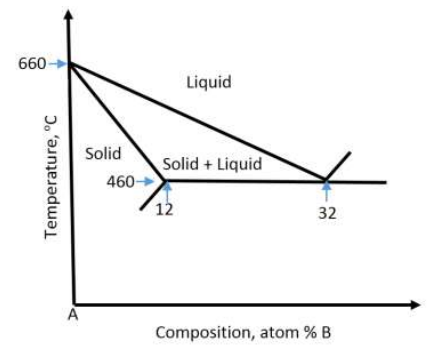
\includegraphics[width=0.5\textwidth]{figures/22.png}
\end{center}
The freezing range of the alloy with 16\% B is \_\_\_\_\_\_\_ (in \(^\circ\)C to one decimal place)}{22}
\vspace{0.5cm}

\questiona{A vector field is given as follows:  

\[
\mathbf{f} = (-x^2 y + x y^2)\,\hat{i} + (x^2 y)\,\hat{j}
\]

The divergence of this field evaluated at \((x, y) = (2, 2)\) is \_\_\_\_\_\_\_\_\_.}{23}
\vspace{0.5cm}

\questiona{A plate of thickness \(h = 120\) mm is cold rolled in a mill with a roll diameter of 200 mm. If the coefficient of friction \(\mu\) is 0.1, the maximum possible reduction \(\Delta h\) in a single pass is \_\_\_\_\_\_\_ (in mm to one decimal place)}{24}
\vspace{0.5cm}

\questiona{A copper-aluminium diffusion couple develops a certain concentration profile after an isothermal treatment at 600\(^\circ\)C for 10 hours. The time required to achieve the same concentration profile at 500\(^\circ\)C is \_\_\_\_\_\_\_ (in hours to 1 decimal place)

Given: The interdiffusion coefficient for copper in aluminium at 500\(^\circ\)C and 600\(^\circ\)C are \(4 \times 10^{-14}\) m\(^2\)/s and \(8 \times 10^{-13}\) m\(^2\)/s.}{25}
\vspace{0.5cm}

\questionb{The molar free energy (J mol\(^{-1}\)) of a liquid solution of a binary A-B alloy as a function of temperature (T) and composition (x, the mole fraction of B) is given by:

\[
G_L(T, x) = (1 - x)G_A^{0,L} + xG_B^{0,L} + RT[x \ln x + (1 - x) \ln(1 - x)] + 4000x(1 - x)
\]

where \(G_A^{0,L}\) and \(G_B^{0,L}\) are the molar free energies of pure liquid A and pure liquid B. What is the excess molar free energy, \(G_{XS,L}\), for an alloy with \(x = 0.5\) at \(T = 1000\,K\)?  

Given: Gas constant \(R = 8.314\, J\, K^{-1}\, mol^{-1}\)}{26}
\begin{enumerate}
    \item[(A)] 1000 J mol\(^{-1}\)  
    \item[(B)] –2000 J mol\(^{-1}\)  
    \item[(C)] 4763 J mol\(^{-1}\)  
    \item[(D)] –5763 J mol\(^{-1}\)  
\end{enumerate}
\vspace{0.5cm}

\questionb{Determine the correctness (or otherwise) of the following Assertion [A] and the Reason [R]:  

\textbf{Assertion [A]:} For a material exhibiting Coble creep, a reduction in grain size results in a significant increase in creep rate.  

\textbf{Reason [R]:} Grain boundaries act as a barrier to motion of dislocations.}{27}
\begin{enumerate}
    \item[(A)] Both [A] and [R] are true and [R] is the correct reason for [A]  
    \item[(B)] Both [A] and [R] are true, but [R] is not the correct reason for [A]  
    \item[(C)] Both [A] and [R] are false  
    \item[(D)] [A] is true but [R] is false  
\end{enumerate}
\vspace{0.5cm}

\questionb{Determine the correctness (or otherwise) of the following Assertion [A] and the Reason [R]:  

\textbf{Assertion [A]:} Refractory BCC metals like W and Mo are less ductile than FCC metals like Ni and Pt at room temperature.  

\textbf{Reason [R]:} BCC metals have fewer independent slip systems than FCC metals.}{28}
\begin{enumerate}
    \item[(A)] Both [A] and [R] are true and [R] is the correct reason for [A]  
    \item[(B)] Both [A] and [R] are true, but [R] is not the correct reason for [A]  
    \item[(C)] Both [A] and [R] are false  
    \item[(D)] [A] is true but [R] is false  
\end{enumerate}
\vspace{0.5cm}

\questionb{A glass fibre of 5 micron diameter is subjected to a tensile stress of 20 MPa. The surface energy and elastic modulus of this material are 0.3 Jm\(^{-2}\) and 70 GPa, respectively. Pick the correct answer based on the information provided above:  

Note: The glass fibre contains a population of flaws of different lengths.}{29}
\begin{enumerate}
    \item[(A)] The fibre will undergo brittle fracture  
    \item[(B)] The fibre will undergo plastic deformation, but not fracture  
    \item[(C)] The fibre will undergo elastic deformation, but not fracture  
    \item[(D)] The fibre will undergo buckling  
\end{enumerate}
\vspace{0.5cm}

\questionb{Two equal and opposite point charges \(+Q\) and \(-Q\) are located as shown in the figure below. A surface integral, \(F_i\) is defined on surface \(S_i\) of a sphere of radius \(r_i\) as follows:  

\[
F_i = \oint_{S_i} (\vec{E} \cdot \hat{n})\, dS
\]

where \(\vec{E}\) is the electric field, and \(\hat{n}\) is the unit normal to the surface of integration.  

If \(r_1 : r_2 : r_3\) are in the ratio 1:2:5, use the Gauss divergence theorem to determine the ratio \(F_1 : F_2 : F_3\).}{30}
\begin{center}
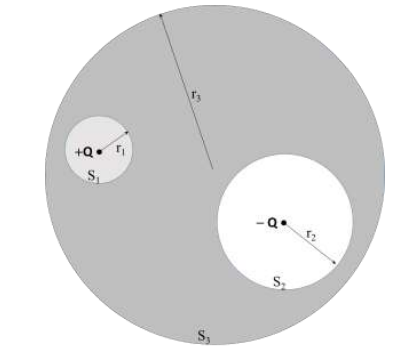
\includegraphics[width=0.5\textwidth]{figures/30.png}
\end{center}
\begin{enumerate}
    \item[(A)] 1 : 2 : 5  
    \item[(B)] 5 : 2 : 1  
    \item[(C)] 1 : –1 : 0  
    \item[(D)] 1 : 1 : 0  
\end{enumerate}
\vspace{0.5cm}

\questionb{Match the four tensile stress-strain curves (P, Q, R, S) with the materials listed in the box:  

1. Polyester (PET)  
2. High purity Copper  
3. Mild Steel  
4. Soda-lime Glass}{31}
\begin{center}
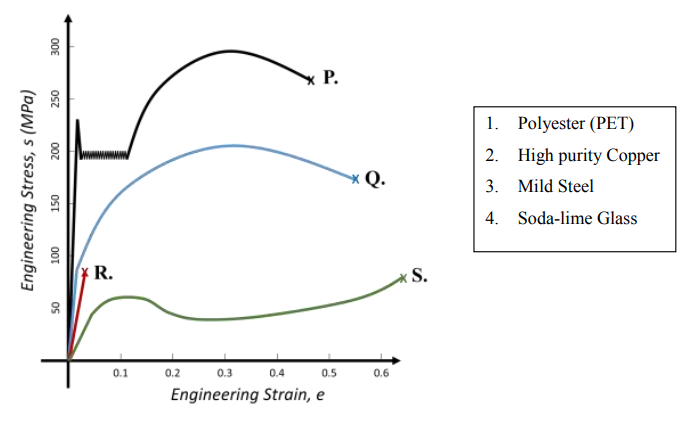
\includegraphics[width=0.5\textwidth]{figures/31.png}
\end{center}
\begin{enumerate}
    \item[(A)] P–1, Q–2, R–3, S–4  
    \item[(B)] P–3, Q–1, R–4, S–2  
    \item[(C)] P–3, Q–2, R–4, S–1  
    \item[(D)] P–2, Q–3, R–4, S–1  
\end{enumerate}
\vspace{0.5cm}

\questionb{Match the metal in Group 1 with the appropriate extractive process in Group 2  

\textbf{Group 1} \hspace{2cm} \textbf{Group 2}  

P. Fe \hspace{2.8cm} 1. Metallothermic Reduction  

Q. Ni \hspace{2.7cm} 2. Carbothermic Reduction  

R. Al \hspace{2.8cm} 3. Matte Smelting  

S. Cr \hspace{2.8cm} 4. Fused Salt Electrolysis}{32}
\begin{enumerate}
    \item[(A)] P–1, Q–2, R–4, S–3  
    \item[(B)] P–2, Q–4, R–1, S–3  
    \item[(C)] P–2, Q–3, R–4, S–1  
    \item[(D)] P–2, Q–1, R–4, S–3  
\end{enumerate}
\vspace{0.5cm}

\questionb{Fe is produced in a reactor using pure \(Fe_2O_3\), C and \(O_2\). For every mole of Fe produced, 2.38 moles of C is used. The exit gas from the reactor contains CO and \(CO_2\) in the molar ratio of 1:1. How many moles of \(O_2\) are consumed for every mole of Fe produced?}{33}
\begin{enumerate}
    \item[(A)] 1.035  
    \item[(B)] 2.072  
    \item[(C)] 0.513  
    \item[(D)] 4.147  
\end{enumerate}
\vspace{0.5cm}

\questionb{What is the voltage required to electrolytically refine impure copper of activity \(a_{Cu} = 0.9\) (Raoultian standard state) to pure copper at 300 K?  

Given: Gas constant \(R = 8.314\, J\, mol^{-1} K^{-1}\), and Faraday’s constant \(F = 96500\, C\, mol^{-1}\).}{34}
\begin{enumerate}
    \item[(A)] 1.36 mV  
    \item[(B)] 2.72 mV  
    \item[(C)] 0 mV  
    \item[(D)] 5.44 mV  
\end{enumerate}
\vspace{0.5cm}

\questionb{Consider the following Ordinary Differential Equation:  

\[
\frac{d}{dx} \left( c \frac{dc}{dx} \right) = 0
\]

In a domain \(0 \leq x \leq t\), with boundary conditions \(c(0) = 0.5\) and \(c(t) = 1.0\), pick the appropriate choice for \(c(x)\) from the following options:}{35}
\begin{center}
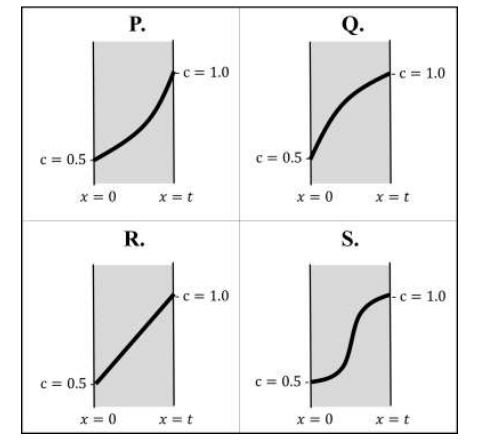
\includegraphics[width=0.5\textwidth]{figures/35.png}
\end{center}
\begin{enumerate}
    \item[(A)] P  
    \item[(B)] Q  
    \item[(C)] R  
    \item[(D)] S  
\end{enumerate}
\vspace{0.5cm}

\questionb{Match the manufacturing processes in Group 1, with the types of cracks in Group 2:

\textbf{Group 1} \hspace{2.5cm} \textbf{Group 2}

P. Arc welding \hspace{2cm} 1. Edge crack  

Q. Extrusion \hspace{2.4cm} 2. Chevron crack  

R. Drawing \hspace{2.5cm} 3. Surface crack  

S. Rolling \hspace{2.5cm} 4. Liquation crack}{36}
\begin{enumerate}
    \item[(A)] P–1, Q–2, R–3, S–4  
    \item[(B)] P–1, Q–3, R–4, S–2  
    \item[(C)] P–4, Q–3, R–2, S–1  
    \item[(D)] P–4, Q–2, R–1, S–3  
\end{enumerate}
\vspace{0.5cm}

\questionb{Consider a dilute substitutional solid solution of X in a metal A. The powder diffraction pattern of this alloy reveals that all the peaks have shifted to the left when compared to those for pure A (with no splitting of peaks). If such a solute interacts and segregates to an edge dislocation, which of the following positions around the dislocation will it preferentially occupy?}{37}
\begin{center}
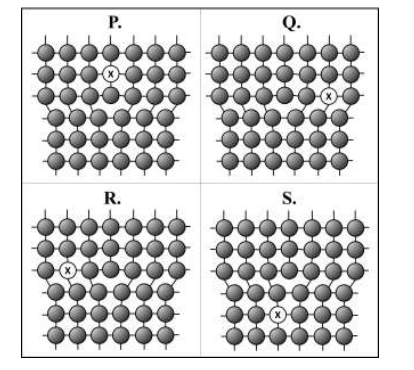
\includegraphics[width=0.5\textwidth]{figures/37.png}
\end{center}
\begin{enumerate}
    \item[(A)] P  
    \item[(B)] Q  
    \item[(C)] R  
    \item[(D)] S  
\end{enumerate}
\vspace{0.5cm}

\questionb{A classroom of 20 students can be categorized on the basis of blood-types: 5 students each with “A”, “B”, “AB”, and “O” blood-types. If four students are selected at random from this class, what is the probability that each student has a different blood-type?}{38}
\begin{enumerate}
    \item[(A)] 0.2500  
    \item[(B)] 0.1289  
    \item[(C)] 0.0625  
    \item[(D)] 0.0156  
\end{enumerate}
\vspace{0.5cm}

\questionb{If the solid-liquid interfacial energy increases by 10\%, the energy barrier for homogeneous nucleation of a spherical solid from the liquid, will change by:}{39}
\begin{enumerate}
    \item[(A)] 21\%  
    \item[(B)] 33\%  
    \item[(C)] –10\%  
    \item[(D)] 46\%  
\end{enumerate}
\vspace{0.5cm}

\questionb{Consider the following stress state imposed on a material:

\[
\sigma = \begin{bmatrix}
90 & 50 & 0 \\
50 & -20 & 0 \\
0 & 0 & 140
\end{bmatrix} \text{MPa}
\]

If the material responds elastically with a volumetric strain \(\Delta = 3.5 \times 10^{-4}\), what is its bulk modulus?}{40}
\begin{enumerate}
    \item[(A)] 150 GPa  
    \item[(B)] 350 GPa  
    \item[(C)] 200 GPa  
    \item[(D)] 400 GPa  
\end{enumerate}
\vspace{0.5cm}

\questionb{A continuous and aligned carbon-fiber composite consists of 25 vol.\% of fibers in an epoxy matrix. The Young’s modulus of fiber and matrix, respectively, are \(E_f = 250\, \text{GPa}\) and \(E_m = 2.5\, \text{GPa}\).  

If the composite is subjected to longitudinal loading (iso-strain condition and assuming elastic response), the fraction of load borne by the reinforcement is \_\_\_\_\_\_\_ (to two decimal places)}{41}
\vspace{0.5cm}

\questionb{Pure iron transforms from body-centered cubic (BCC) to face-centered cubic (FCC) crystal structure at 912\(^\circ\)C. If the lattice parameter of the BCC phase is 0.293 nm and that of the FCC phase is 0.363 nm, the associated volume change is \_\_\_\_\_\_\_ (in \% to one decimal place)}{42}
\vspace{0.5cm}

\questionb{As shown in the schematic below, an alloy is cast as a rectangular slab between two thick mould walls that differ in their thermal conductivities. Shrinkage defects are found at a distance \(L_1\) from Mould-1 with thermal conductivity \(k_1\) and distance \(L_2\) from Mould-2 with thermal conductivity \(k_2\). If the ratio \(L_1 : L_2 = 3 : 2\), and assuming 1-D heat transfer, the ratio \((k_1 / k_2)\) is \_\_\_\_\_\_\_ (to two decimal places)}{43}
\begin{center}
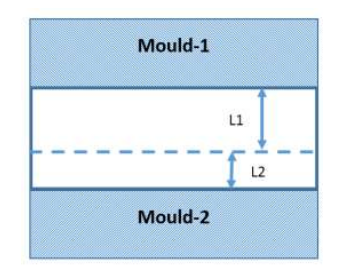
\includegraphics[width=0.5\textwidth]{figures/43.png}
\end{center}
\vspace{0.5cm}

\questionb{The temperature profile (\(T\) in Kelvin) of an arc weld across its width is given as  
\[ T = 2000 \exp(-0.3x^2) \]  
where \(x\) (in mm) is the distance from the weld centre. The melting point of the base material is 1500 K. The width of the fusion zone is \_\_\_\_\_\_\_ (in mm to two decimal places).}{44}
\vspace{0.5cm}

\questionb{The terminal velocity (\(v\)) of a spherical inclusion of diameter \(D = 50\) micrometers rising in liquid steel is \_\_\_\_\_\_\_ (in mm/s to two decimal places)  

Assume Stokes law; i.e., drag force \(F_d = 3\pi\mu D v\), where \(\mu\) is the viscosity of steel.  

Given:  
Density of liquid steel = 7900 kg/m\(^3\)  
Viscosity of liquid steel = 0.0079 Pa·s  
Density of the inclusion = 2500 kg/m\(^3\)  
Acceleration due to gravity = 9.8 m/s\(^2\)}{45}
\vspace{0.5cm}

\questionb{A single crystal of aluminium is subjected to 10 MPa tensile stress along the [321] crystallographic direction. The resolved shear stress on the \((1\bar{1}1)\)[101] slip system is \_\_\_\_\_\_\_ (in MPa to two decimal places).}{46}
\vspace{0.5cm}

\questionb{If the net magnetic moment of an Fe atom in BCC structure is \(2\,\mu_B\), then the saturation magnetization of Fe is \_\_\_\_\_\_\_ (kA/m to one decimal place)  

Given: \(\mu_B = 9.273 \times 10^{-24}\, \text{A·m}^2\); Lattice parameter of BCC iron = 0.287 nm  

Note: kA is kiloAmperes.}{47}
\vspace{0.5cm}

\questionb{If 2 moles of Au and 3 moles of Ag are mixed to form a single-phase ideal solid solution, the total entropy of mixing is \_\_\_\_\_\_\_ (in J/K to one decimal place)  

Given: Gas constant \(R = 8.314\, \text{J/K·mol}\)}{48}
\vspace{0.5cm}

\questionb{A spherical liquid metal droplet of diameter 1 mm is solidified in a stream of gas at 300 K. Assuming that the metal droplet remains at its melting point of 900 K and neglecting radiative losses, the time to complete the solidification is \_\_\_\_\_\_\_ (in seconds to one decimal place).  

Given:  
Enthalpy of fusion = 4000 kJ/kg  
Convective heat transfer coefficient = 200 W/m\(^2\cdot\)K  
Density of liquid metal = 2700 kg/m\(^3\)}{49}
\vspace{0.5cm}

\questionb{At a temperature of 710 K, the vapour pressure of pure liquid Zn is given by:  
\[ p_{\text{Zn}}(X_{\text{Zn}} = 1.0) = 3.6 \times 10^{-4}\, \text{atm} \]  

The Raoultian activity coefficient \((\gamma_{\text{Zn}})\) of Zn in Zn-Cd alloy liquid at 710 K is approximated by:  
\[
\ln(\gamma_{\text{Zn}}) = 0.875(1 - X_{\text{Zn}})^2
\]

The ratio \( \left[ \frac{p_{\text{Zn}}(X_{\text{Zn}} = 0.7)}{p_{\text{Zn}}(X_{\text{Zn}} = 1.0)} \right] \) is \_\_\_\_\_\_\_ (to two decimal places)}{50}
\vspace{0.5cm}

\questionb{For the reaction:  
\[ 4Ag(s, \text{pure}) + O_2(g) \rightarrow 2Ag_2O(s, \text{pure}) \]  
the standard enthalpy change, \(\Delta H^0 = -61080\, \text{J}\), and the standard entropy change, \(\Delta S^0 = -132.22\, \text{J/K}\), in the temperature range from 298 K to 500 K.  

The temperature above which \(Ag_2O\) decomposes in an atmosphere containing oxygen at a partial pressure \(p_{O_2} = 0.3\) atm is \_\_\_\_\_\_\_ (in K to one decimal place).  

Given: Gas constant \(R = 8.314\, \text{J/K·mol}\)}{51}
\vspace{0.5cm}

\questionb{In a powder diffraction experiment on BCC iron, the first peak occurs at \(2\theta = 68.7^\circ\). The wavelength of X-rays is \_\_\_\_\_\_\_ (in nm to three decimal places).  

Given: Lattice parameter of iron = 0.287 nm}{52}
\vspace{0.5cm}

\questionb{A 1 mol piece of copper at 400 K is brought in contact with another 1 mol piece of copper at 300 K, and allowed to reach thermal equilibrium. The entropy change for this process is \_\_\_\_\_\_\_ (in J/K to three decimal places).  

Given: Specific heat capacity of copper (between 250 K and 500 K) is 22.6 J/K·mol  

Assume that the system containing the two pieces of copper remains isolated during this process.}{53}
\vspace{0.5cm}

\questionb{Using the trapezoidal rule with two equal intervals (n = 2, \(\Delta x = 1\)), the definite integral  
\[
\int_{2}^{4} \ln(x) \, dx = \_\_\_\_\_\_\_
\]  
(to two decimal places)}{54}
\vspace{0.5cm}

\questionb{The ideal plastic work involved in extruding a cylindrical billet of length 100 mm, from an initial diameter of 20 mm to a final diameter of 16 mm is \_\_\_\_\_\_\_ (in J to one decimal place).  

The flow stress in compression is 40 MPa and remains constant throughout the process.}{55}
\vspace{0.5cm}

\vspace{5cm}
\begin{center}
\textbf{END OF THE QUESTION PAPER} \\
\rule{\textwidth}{0.5pt}
\end{center}

\end{document}
